\documentclass{article}

\usepackage{tikz} 
\usetikzlibrary{automata, positioning, arrows} 

\usepackage{amsthm}
\usepackage{amsfonts}
\usepackage{amsmath}
\usepackage{amssymb}
\usepackage{fullpage}
\usepackage{color}
\usepackage{parskip}
\usepackage{hyperref}

  \hypersetup{
    colorlinks = true,
    urlcolor = blue,       % color of external links using \href
    linkcolor= blue,       % color of internal links 
    citecolor= blue,       % color of links to bibliography
    filecolor= blue,        % color of file links
    }
    
\usepackage{listings}

\definecolor{dkgreen}{rgb}{0,0.6,0}
\definecolor{gray}{rgb}{0.5,0.5,0.5}
\definecolor{mauve}{rgb}{0.58,0,0.82}

\lstset{frame=tb,
  language=haskell,
  aboveskip=3mm,
  belowskip=3mm,
  showstringspaces=false,
  columns=flexible,
  basicstyle={\small\ttfamily},
  numbers=none,
  numberstyle=\tiny\color{gray},
  keywordstyle=\color{blue},
  commentstyle=\color{dkgreen},
  stringstyle=\color{mauve},
  breaklines=true,
  breakatwhitespace=true,
  tabsize=3
}

\newtheoremstyle{theorem}
  {\topsep}   % ABOVESPACE
  {\topsep}   % BELOWSPACE
  {\itshape\/}  % BODYFONT
  {0pt}       % INDENT (empty value is the same as 0pt)
  {\bfseries} % HEADFONT
  {.}         % HEADPUNCT
  {5pt plus 1pt minus 1pt} % HEADSPACE
  {}          % CUSTOM-HEAD-SPEC
\theoremstyle{theorem} 
   \newtheorem{theorem}{Theorem}[section]
   \newtheorem{corollary}[theorem]{Corollary}
   \newtheorem{lemma}[theorem]{Lemma}
   \newtheorem{proposition}[theorem]{Proposition}
\theoremstyle{definition}
   \newtheorem{definition}[theorem]{Definition}
   \newtheorem{example}[theorem]{Example}
\theoremstyle{remark}    
  \newtheorem{remark}[theorem]{Remark}

\title{CPSC-354 Report}
\author{Sarah Yoon  \\ Chapman University}

\date{\today} 

\begin{document}

\maketitle

\begin{abstract}

\end{abstract}

\setcounter{tocdepth}{3}
\tableofcontents

\section{Introduction}\label{intro}

\section{Week by Week}\label{homework}

\subsection{Week 1}

\subsubsection*{Notes}
Learned about some tactics and theorems

rfl: a tactic that proves theorems that take the form of X = X \\
rw: a tactic that rewrites a proof\\
one\_eq\_succ\_zero: a theorem that proves 1 = succ 0 (there are also other similar existing theorems like two\_eq\_succ\_one and so on)\\
add\_zero: a theorem that proves a + 0 = a.\\
add\_succ: a theorem that proves a + succ b = succ(a + b)\\
succ\_eq\_add\_one: a theorem that proves succ a = a + 1\\

\subsubsection*{Homework}
Problem 5: \\
a b c are in the set of natural numbers. \\
Prove that both sides are equal to each other. \\
a + (b + 0) + (c + 0) = a + b + c \\
rw [add\_zero] - uses the add\_zero theorem to prove that b + 0 = b \\
This is rewritten to: \\
a + b + (c + 0) = a + b + c \\
rw [add\_zero] - this is done again to prove that c + 0 = c \\ 
This is rewritten to: \\
a + b + c = a + b + c \\
rfl - this proves that both sides that look the same are equal to each other \\

Problem 6: \\
This is the same problem as 5 but will be approached in a different manner. \\
a + (b + 0) + (c + 0) = a + b + c \\
rw [add\_zero c] - specifically applies the add\_zero theorem to c, making c + 0 into c \\
This is rewritten to: \\ 
a + (b + 0) + c = a + b + c \\
rw [add\_zero b] - specifically applies the add\_zero theorem to b, making b + 0 into b \\
This is rewritten to: \\ 
a + b + c = a + b + c \\
rfl - this proves that both sides that look the same are equal to each other \\

Problem 7: \\
n is in the set of natural numbers. \\
Prove that both sides are equal to each other. \\
succ n = n + 1
rw[one\_eq\_succ\_zero] - rewrite 1 into successor 0
This is rewritten to: \\ 
succ n = n + succ 0 \\
rw[add\_succ] - uses the add\_succ theorem to change n + succ 0 into succ(n + 0) \\
This is rewritten to: \\ 
succ n = succ (n + 0) \\
rw[add\_zero] - uses the add\_zero theorem to prove that n + 0 = n \\
This is rewritten to: \\ 
succ n = succ n \\
rfl - this proves that both sides that look the same are equal to each other \\

Problem 8: \\
Prove that both sides are equal to each other. \\
2 + 2 = 4 \\
rw[two\_eq\_succ\_one] - rewrites 2 into succ 1 \\
This is rewritten to: \\ 
succ 1 + succ 1 = 4 \\
rw[one\_eq\_succ\_zero] - rewrites 1 into succ 0 \\
This is rewritten to: \\ 
succ (succ 0) + succ (succ 0) = 4 \\
rw[four\_eq\_succ\_three] - rewrites 4 into succ 3 \\
This is rewritten to: \\ 
succ (succ 0) + succ (succ 0) = succ 3 \\
rw[three\_eq\_succ\_two] - rewrites 3 into succ 2 \\
This is rewritten to: \\ 
succ (succ 0) + succ (succ 0) = succ (succ 2) \\
rw[two\_eq\_succ\_one] - rewrites 2 into succ 1 \\
This is rewritten to: \\ 
succ (succ 0) + succ (succ 0) = succ (succ (succ 1)) \\
rw[one\_eq\_succ\_zero] - rewrites 1 into succ 0 \\
This is rewritten to: \\ 
succ (succ 0) + succ (succ 0) = succ (succ (succ (succ 0))) \\
rw[add\_succ] - changes succ (succ 0) + succ (succ 0) into succ (succ (succ 0) + succ 0) \\
This is rewritten to: \\ 
succ (succ (succ 0) + succ 0) = succ (succ (succ (succ 0))) \\
rw[add\_succ] - changes succ (succ (succ 0) + succ 0) into succ (succ (succ (succ 0) + 0)) \\
This is rewritten to: \\ 
succ (succ (succ (succ 0) + 0)) = succ (succ (succ (succ 0))) \\
rw[add\_zero] - changes succ (succ 0) + 0 into \\
This is rewritten to: \\ 
succ (succ (succ (succ 0))) = succ (succ (succ (succ 0))) \\ 
rfl - this proves that both sides that look the same are equal to each other \\

For level 5: 
add\_zero is a Lean proof that a + 0 = a (a representing any number). In mathematics, there are laws for arithemic. One of them 
is called the identity which applies to addition and multiplication. For addition, it states that m + 0 = m = 0 + m. This is the
exact same as the Lean proof, a + 0 = a, which can also be written as a = 0 + a.

%In case you want to draw automata in Latex, you can use the tikz %package. Here is an example of a simple automaton:
%
%\begin{tikzpicture}[shorten >=1pt,node distance=2cm,on grid,auto] 
%  \node[state] (q_1)   {$q_1$}; 
%  \node[state] (q_2) [above right=of q_1] {$q_2$}; 
%  \node[state] (q_3) [below right=of q_2] {$q_3$}; 
%   \path[->] 
%   (q_1) edge  node {0} (q_2)
%         edge  node [swap] {1} (q_3)
%   (q_2) edge  node  {1} (q_3)
%         edge [loop above] node {0} ()
%   (q_3) edge [loop below] node {0,1} ();
%\end{tikzpicture}
%
%By the way, GPT-4 is quite good at outputting tikz code.

\subsubsection*{Comments and Questions}
Learning the root of mathematics is very eye-opening, and I am confident it will be the same for programming languages. 
It provides another perspective for elementary functions like 2 + 2 equals 4, which is different from just knowing it through memorization. 
I feel as though this is why people have been able to expand mathematically. This makes me wonder: how can looking through the core of 
programming help us better current languages (e.g. python, rust)?
%I expect you to read the lecture notes. 

\subsection{Week 2}

\subsubsection*{Notes}
Recursion as a concept using the Towers of Hanoi:
It is broken down into:
 moving a tower of n disks from x to y
 moving a tower of n+1 disks when it is already known how to move a tower of n disks
The algorithm is made up of a bunch of "pushs" and "pops"
The logic overall is a bunch of back and forth movement of the disks 

Lean:
induction proof with: induction n with d hd
succ\_add: proves that succ a + b = succ (a + b)
add\_comm x y: proves that x + y = y + x
add\_assoc: proves that a + b + c = a + (b + c)
add\_right\_comm a b c: proves that a + b + c = a + c + b 

\subsubsection*{Homework}
Problem 1:\\
n is in the natural number set\\
Prove 0 + n = n.\\
induction n with d hd - starting a proof by induction\\
Now our first goal is:\\
0 + 0 = 0\\
rw[add\_zero] - proves that 0 + 0 = 0\\
This is rewritten to:\\
0 = 0\\
rfl - this proves that both sides that look the same are equal to each other \\
Now, we prove our second goal\\
hd: 0 + d = d\\
0 + succ d = succ d \\
rw[add\_succ] - proves that 0 + succ d = succ (0 + d)\\
This is rewritten to:\\
succ (0 + d) = succ d\\
rw[hd] - this replaces 0 + d with d\\
This is rewritten to:\\
succ d = succ d\\
rfl - this proves that both sides that look the same are equal to each other \\

Problem 2:\\
a b is in the set of natural numbers\\
Prove succ a + b = succ (a + b)\\
inductin b with d hd - starting a proof by induction\\
Now our first goal is:\\
succ a + 0 = succ (a + 0)\\
rw[add\_zero] - proves that succ a + 0 = succ a\\
This is rewritten to:\\
succ a = succ(a + 0)\\
rw[add\_zero] - proves that succ (a + 0) = succ a\\
This is rewritten to:\\
succ a = succ a\\
rfl - this proves that both sides that look the same are equal to each other \\
Now, we prove our second goal\\
hd: succ a + d = succ (a + d)\\
succ a + succ d = succ (a + succ d)\\
rw[add\_succ] - proves that succ a + succ d = succ (succ a + d)\\
This is rewritten to:\\
succ (succ a + d) = succ (a + succ d)\\
rw[hd] - this replaces succ a + d with succ (a + d)\\
This is rewritten to:\\
succ (succ (a + d)) = succ (a + succ d)\\
rw[add\_succ] - proves that succ (a + succ d) = succ (succ (a + d))\\
This is rewritten to:\\
succ (succ (a + d)) = succ (succ (a + d))\\
rfl - this proves that both sides that look the same are equal to each other \\

Problem 3:\\
a b is in the set of natural numbers\\
Prove a + b = b + a\\
induction b with hd - starting a proof by induction\\
Now our first goal is:\\
a + 0 = 0 + a\\
rw[zero\_add] - proves that 0 + a = a\\
This is rewritten to:\\
a + 0 = a\\
rw[add\_zero] - proves that a + 0 = a\\
This is rewritten to:\\
a = a\\
rfl - this proves that both sides that look the same are equal to each other \\
Now, we prove our second goal\\
n\_ih: a + hd = hd + a\\
a + succ hd = succ hd + a\\
rw[add\_succ] - proves that a + succ hd = succ (a + hd)\\
This is rewritten to:\\
succ (a + hd) = succ hd + a\\
rw[succ\_add] - proves that succ hd + a = succ (hd + a)\\
This is rewritten to:\\
succ (a + hd) = succ (hd + a)\\
rw[n\_ih] - replaces succ (a + hd) with succ (hd + a)\\
This is rewritten to:\\
succ (hd + a) = succ (hd + a)\\
rfl - this proves that both sides that look the same are equal to each other \\

Problem 4:\\
a b c is in the set of natural numbers\\
Prove a + b + c = a + (b + c)\\
induction a with hd - starting a proof by induction\\
Now our first goal is:\\
0 + b + c = 0 + (b + c)\\
rw[zero\_add] - proves that 0 + b = b\\
This is rewritten to:\\
b + c = 0 + (b + c)\\
rw[zero\_add] - proves that 0 + (b + c) = b + c\\
This is rewritten to:\\
b + c = b + c\\
rfl - this proves that both sides that look the same are equal to each other \\
Now, we prove our second goal\\
n\_ih: hd + b + c = hd + (b + c)\\
succ hd + b + c = succ hd + (b + c)\\
rw[succ\_add] - proves that succ hd + b + c = succ (hd + b) + c\\
This is rewritten to:\\
succ (hd + b) + c = succ hd + (b + c)\\
rw[succ\_add] - proves that succ (hd + b) + c = succ (hd + b + c)\\
This is rewritten to:\\
succ (hd + b + c) = succ hd + (b + c)\\
rw[n\_ih] - replaces succ (hd + b + c) with succ (hd + (b + c))\\
This is rewritten to:\\
succ (hd + (b + c)) = succ hd + (b + c)\\
rw[succ\_add] - proves succ hd + (b + c) = succ (hd + (b + c))\\
This is rewritten to:\\
succ (hd + (b + c)) = succ (hd + (b + c))\\
rfl - this proves that both sides that look the same are equal to each other \\

Problem 5:\\
a b c is in the set of natural numbers\\
Prove a + b + c = a + c + b\\
induction c with hd - starting a proof by induction\\
Now our first goal is:\\
a + b + 0 = a + 0 + b\\
rw[add\_zero] - proves that b + 0 = b\\
This is rewritten to:\\
a + b = a + 0 + b\\
rw[add\_zero] 0 proves that a + 0 = a\\
This is rewritten to:\\
a + b = a + b\\
rfl - this proves that both sides that look the same are equal to each other \\
Now, we prove our second goal\\
n\_ih: a + b + hd = a + hd + b\\
a + b + succ hd = a + succ hd + b\\
rw[add\_succ] - proves that a + b + succ hd = succ (a + b + hd)\\
This is rewritten to:\\
succ (a + b + hd) = a + succ hd + b\\
rw[add\_succ] - proves that a + succ hd + b = succ (a + hd) + b\\
This is rewritten to:\\
succ (a + b + hd) = succ (a + hd) + b\\
rw[succ\_add] - proves that succ (a + hd) + b = succ (a + hd + b)\\
This is rewritten to:\\
succ (a + b + hd) = succ (a + hd + b)\\
rw[n\_ih] - replaces a + b + hd with a + hd + b\\
This is rewritten to\\
succ (a + hd + b) = succ (a + hd + b)\\
rfl - this proves that both sides that look the same are equal to each other \\

Problem 5 Proof in Mathematics:\\
a + b + c =  a + (b + c)\\
0 + b + c = 0 + (b + c) - Basis\\
b + c = 0 + (b + c) - Addition Identity\\
b + c = b + c - Addition Identity\\
Inductive Step:\\
k + b + c = k + (b + c)\\
The goal is to prove that Sk + b + c = Sk + (b + c)\\
S(k + b + c) = Sk + (b + c) - Definition of Addition\\
S(k + b + c) = S(k + (b + c)) - Definition of Addition\\
S(k + (b + c)) = S(k + (b + c)) - Inductive Hypothesis\\
Therefore, by the Axiom of induction a + b + c =  a + (b + c) for all a in the natural numbers set\\
\\
Math to Lean\\
Basis: induction a with hd\\
Addition Identity: zero\_add\\
Definition of Addition: succ\_add\\
Inductive Hypothesis: n\_ih\\

\subsubsection*{Comments and Questions}
The Towers of Hanoi reminded me of solving certain problems by simply using recursion. 
I also remember applying this method to the Fibonacci sequence. This makes me wonder 
how it transfers to math. How does recursion 
appear in mathematics or, specifically, in Lean?

\subsection{Week 3}

\subsubsection*{Homework}
\href{https://github.com/sarah-yoon/CPSC354_Week3/blob/main/README.md}{Week 3 Assignment}\\
\subsubsection*{Comments and Questions}
My literature review is about the cause for many different programming languages, the abstraction of them in the future, and what needs future ones would need to fulfill. 
I found that languages evolved depending on the different needs and users over time. For instance, Domain-specific languages were created to meet specific needs. SQL, being one of them, was created to interact with databases.
Within the topic of abstraction, PLs are bound to become higher level to not worry about lower-level implementation. Examples of the current progress towards abstraction would be AI-assisted programming and declarative programming. 
However, abstraction will not change the usage of current languages like Java, Python, and C++ in the foreseeable future. These languages have made a huge impact and it is shown through their extensive ecosystems and sheer amount of existing codebases. On the other hand, some specific areas use newer languages like Rust and Kotlin. They fulfill more modern needs like memory safety and developer productivity.
Future programming languages would need to deal with challenges like security, AI, and concurrency.

\subsection{Week 4}
\subsubsection*{Homework}
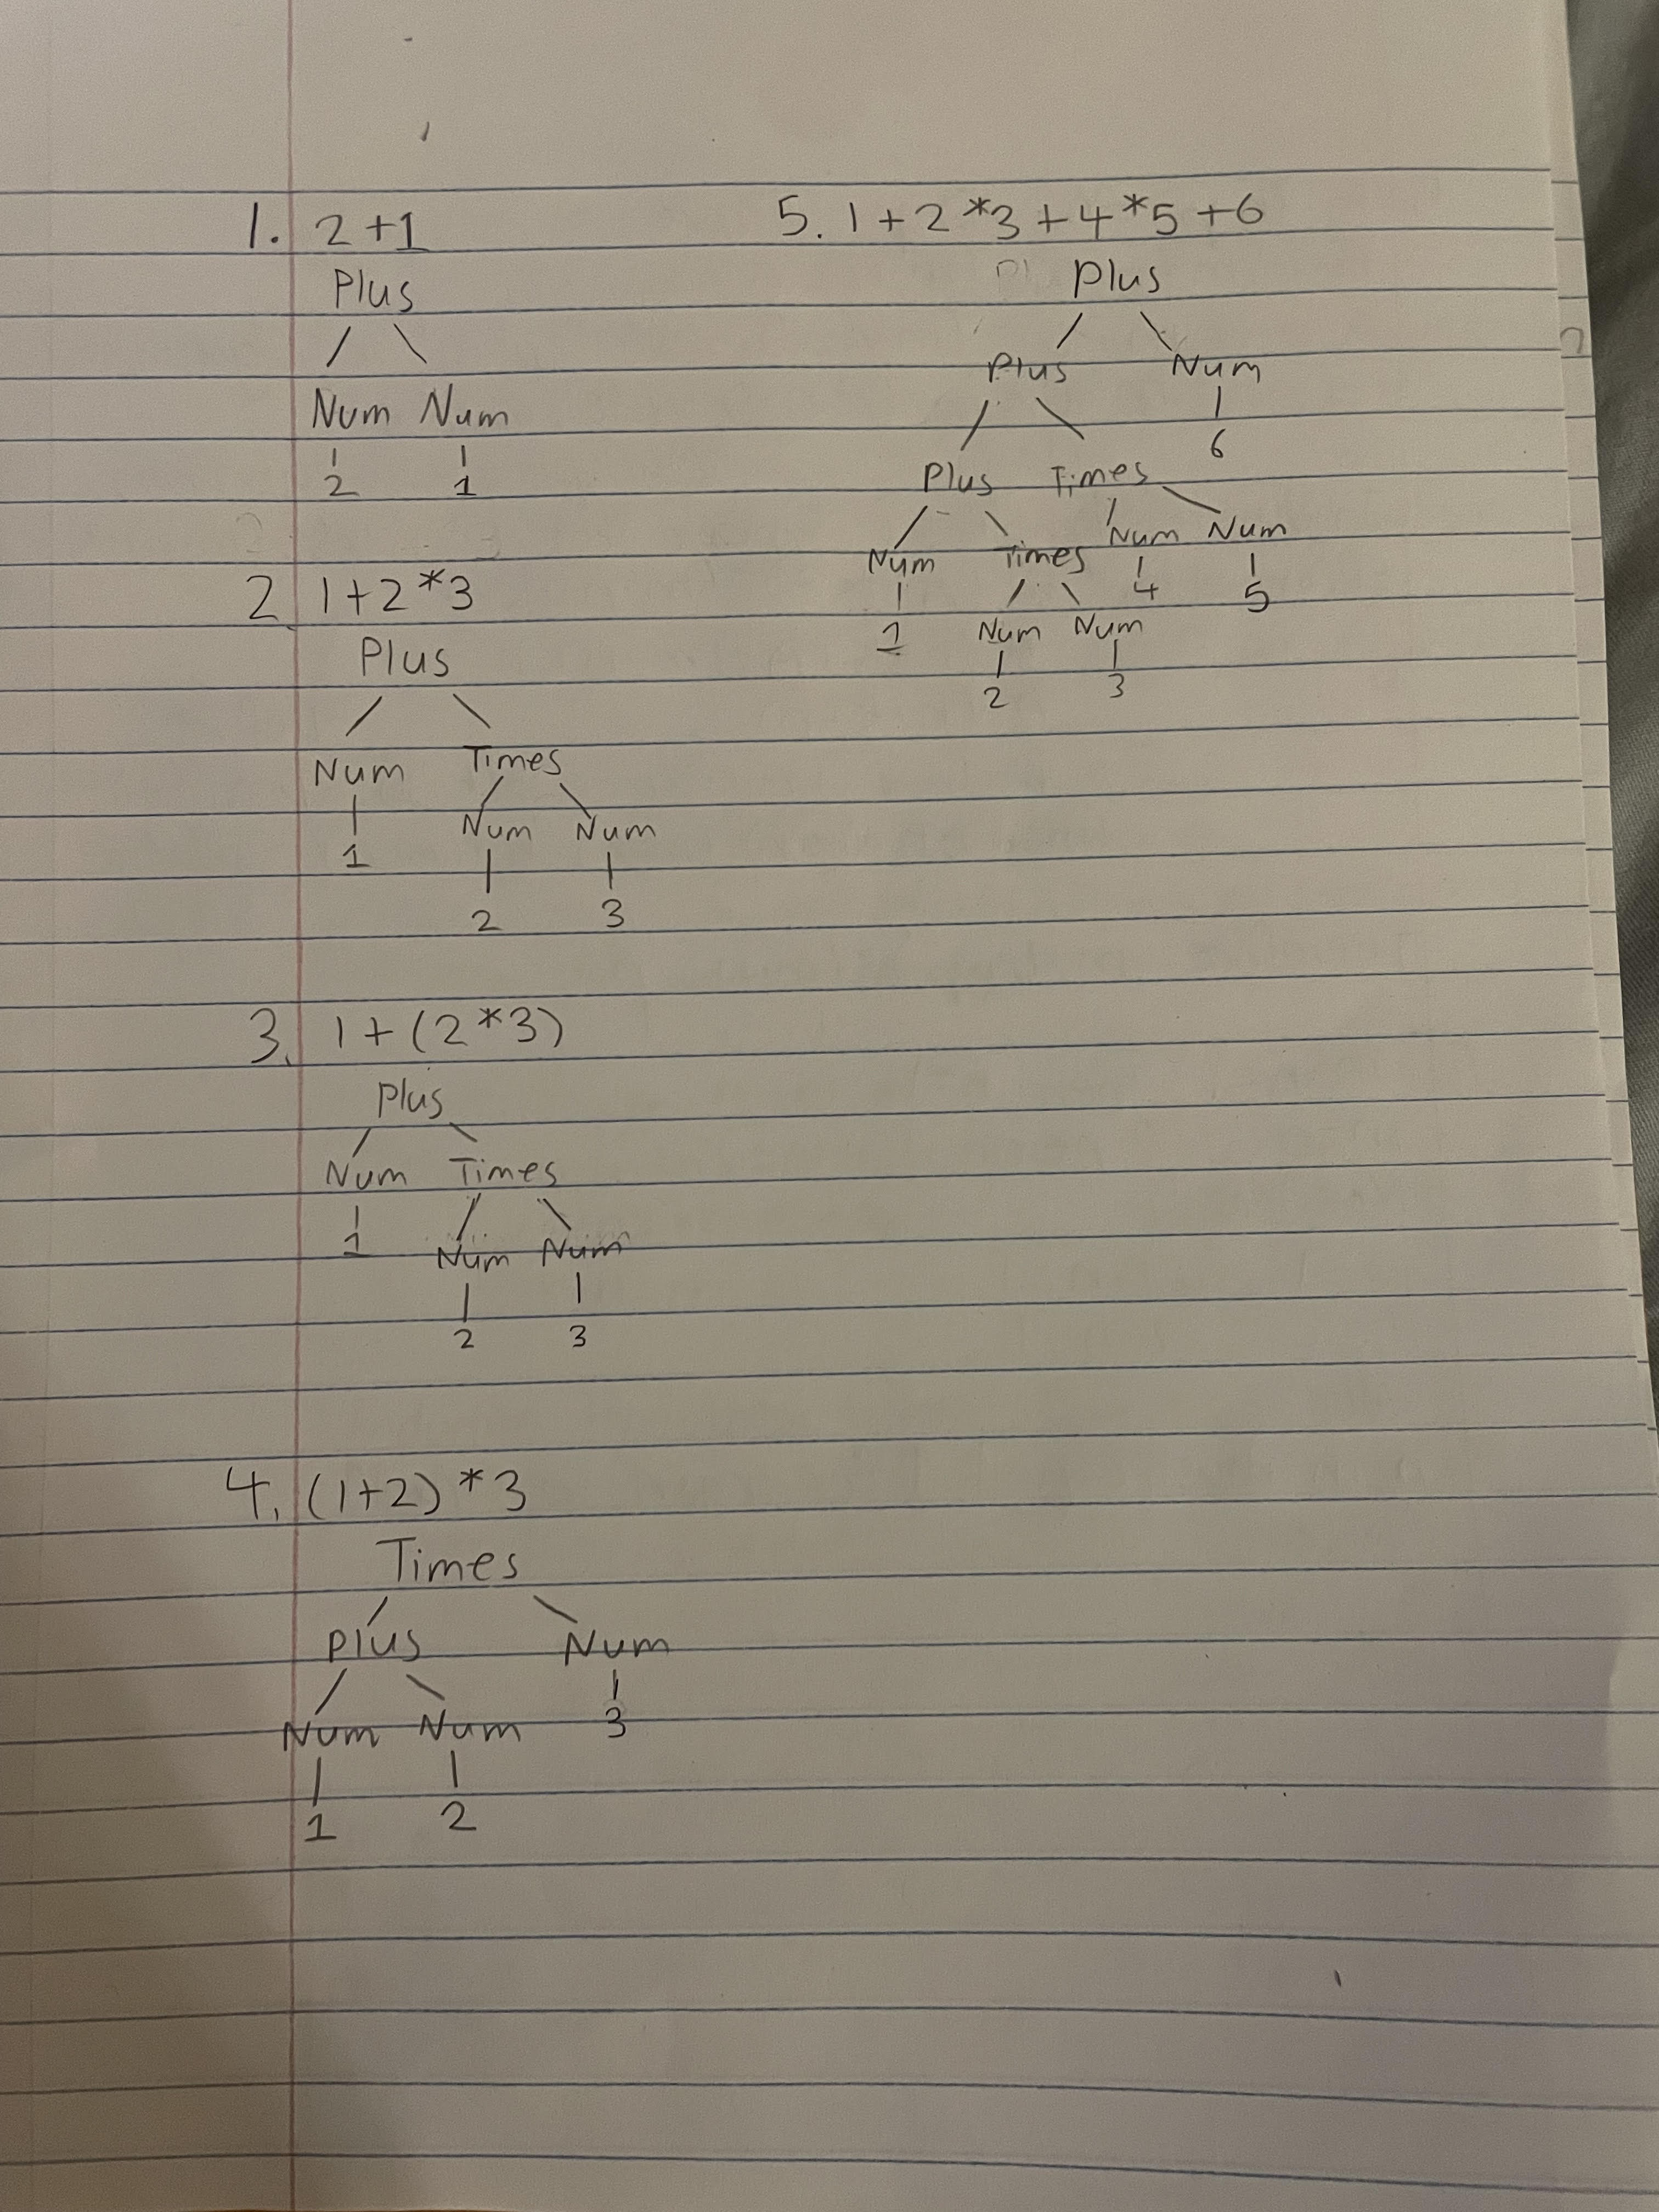
\includegraphics[scale=0.1]{parsing.jpg}
\subsubsection*{Comments and Questions}
Parsing seemed to work really great with expressions. In general, is parsing a good strategy when it comes to breaking things down?

\subsection{Week 5}
\subsubsection*{Notes}
exact -conclusion of a proof\\
Operator: $\land$ -Logical And\\
Example: $A \land B$ -A and B\\
and\_into -takes two pieces of evidence and combines it into one\\
have -adds new assumptions to the proof\\

\subsubsection*{Homework}
Problem 1:\\
exact todo\_list\\

Problem 2:\\
exact and\_intro p s \\

Problem 3:\\
exact ⟨⟨a,i⟩,⟨o,u⟩⟩\\

Problem 4:\\
have p := and\_left vmS\\
exact p\\

Problem 5:\\
have q := and\_right h\\
exact q\\

Problem 6:\\
have a := and\_left h1\\
have u := and\_right h2\\
exact ⟨a, u⟩\\

Problem 7:\\
have h1 := h.left \\
have h2 := h1.right \\
have h3 := h2.left \\
have h4 := h3.left \\
have h5 := h4.right \\
exact h5 \\

Problem 8:\\
have h1 := h.left \\
have a := h1.right\\
have h2 := h1.left\\
have p := h2.left\\
have s := h2.right\\
have h3 := h.right\\
have h4 := h3.right\\
have h5 := h4.left\\
have c := h5.left\\

In mathmatical proof:\\
If $((P \land S) \land A) \land ¬I \land (C \land ¬O) \land ¬U$ then $A \land C \land P \land S$. \\
Proof:\\
(1)\\
$((P \land S) \land A) \land ¬I \land (C \land ¬O) \land ¬U$\\
assumption\\

(2)\\
$(P \land S) \land A$\\
and\_left (1)

(3)\\
A\\
and\_right (2)\\

(4)\\
$(P \land S)$\\
and\_left (2)\\

(5)\\
P\\
and\_left (4)\\

(6)\\
S\\
and\_right (4)\\

(7)\\
$¬I \land (C \land ¬O) \land ¬U$\\
and\_right (1)\\

(8)\\
$(C \land ¬O) \land ¬U$\\
and\_right (7)\\

(9)\\
$C \land ¬O$\\
and\_left (8)\\

(10)\\
C\\
and\_left (9)\\

(11)\\
$A \land C \land P \land S$\\
and\_intro (3)(10)(5)(6)\\

\subsubsection*{Comments and Questions}
How does lean help with problem solving when it comes to programming?\\

\subsection{Week 6}
\subsubsection*{Homework}
Problem 1:\\
have b := bakery\_service p\\
exact b\\

Problem 2:\\
exact fun h : $C =>$ h\\

Problem 3:\\
exact fun $h =>$ and\_intro h.right h.left\\

Problem 4:\\
exact fun h : $C =>$ have a : A := h1 h; h2 a\\

Problem 5:\\
have q : Q := h1 p\\
have t : T := h3 q\\
exact h5 t\\
               
Problem 6:\\
exact fun c : $C =>$\\
  fun d : $D =>$\\
    have cd : $C \land D$ := ⟨c, d⟩;\\
    h cd    \\
    
Couldn't finish...

\subsubsection*{Comments and Questions}
Solving lean logic game is a simple view into proving theorems and the foundations of programming languages. When it comes to the lambda problems specifically, how do real-world challenges complicate the applications of lambda?

\subsection{Week 7}
\subsubsection*{Homework}
1.\\
\[
((\lambda m. \lambda n. m \, n) \, (\lambda f. \lambda x. f \, (f \, x))) \, (\lambda f. \lambda x. f \, (f \, (f \, x)))
\]

\[
((\lambda m. \lambda n. m \, n) \, (\lambda f. \lambda x. f \, (f \, x))) \rightarrow \lambda n. (\lambda f. \lambda x. f \, (f \, x)) \, n
\]

\[
(\lambda f. \lambda x. f \, (f \, x)) \, n \rightarrow \lambda x. n \, (n \, x)
\]

\[
(\lambda n. \lambda x. n \, (n \, x)) \, (\lambda f. \lambda x. f \, (f \, (f \, x)))
\]

\[
(\lambda n. \lambda x. n \, (n \, x)) \, (\lambda f. \lambda x. f \, (f \, (f \, x))) \rightarrow \lambda x. (\lambda f. \lambda x. f \, (f \, (f \, x))) \, ((\lambda f. \lambda x. f \, (f \, (f \, x))) \, x)
\]

\[
(\lambda f. \lambda x. f \, (f \, (f \, x))) \, x \rightarrow \lambda x. x \, (x \, (x \, x))
\]

\[
\lambda x. (\lambda f. \lambda x. f \, (f \, (f \, x))) \, (\lambda x. x \, (x \, (x \, x)))
\]

\[
(\lambda f. \lambda x. f \, (f \, (f \, x))) \, (\lambda x. x \, (x \, (x \, x))) \rightarrow \lambda x. (\lambda x. x \, (x \, (x \, x))) \, ((\lambda x. x \, (x \, (x \, x))) \, x)
\]

\[
(\lambda x. x \, (x \, (x \, x))) \, x \rightarrow x \, (x \, (x \, x))
\]

\[
\lambda x. (\lambda x. x \, (x \, (x \, x))) \, (x \, (x \, (x \, x)))
\]

\[
(\lambda x. x \, (x \, (x \, x))) \, (x \, (x \, (x \, x))) \rightarrow (x \, (x \, (x \, x))) \, ((x \, (x \, (x \, x))) \, ((x \, (x \, (x \, x))) \, (x \, (x \, (x \, x))))
\]

2.\\
The lambda term implements addition on natural numbers. It is done by combing two Church numerals. It carries out addition by counting the the total number of times the function is being applied. 
\subsubsection*{Comments and Questions}
Can church numerals be used to represent recursive functions/processes?

\subsection{Week 8}
\subsubsection*{Homework}
Answers on week 9
\subsubsection*{Comments and Questions}
When it comes to evaluation strategies in lambda calculus, what are the trade-offs? How do these strategies affect performance and accuracy in a practical implementation?

\subsection{Week 9}
\subsubsection*{Homework}
2. a is applied to b, which leads to (ab). Then, (ab) is applied to c, resulting in ((ab)c). Finally, ((ab)c) is applied to d, which leads to (((ab)c)d). (a) reduces to a it's already in its simplest form.

3.When substituting a variable, wall instances of that variable are replaced. However, if the variable being substituted for is also bound, the meaning of the expression is changed. This is implemented by traversing the AST of the expression, checking for bound variables, and renaming them.

4. No, not everything is the expected result.

5. \[Y=\lambda f.(\lambda x.f(xx))(\lambda x.f(xx))\]

\subsubsection*{Comments and Questions}
How could different evaluation strategies impact the trace output produced by an interpreter?

\subsection{Week 10}
\subsubsection*{Homework}
1. The challenge of working through Homework 8/9 and Assignment 3 was figuring out why the interpreter wouldn't completely evaluate everything.

2. The key insight for Assignment 3 was just looking through the evaluation function and looking at where ecxactly it stopped evaluating the function and just returned whatever it found.

3. The most interesting take away was from the homework and assignment was using the debugger to see how far the program would evaluate a lambda function. I never really use the debugger, so it was interesting to break things apart.
\subsubsection*{Comments and Questions}
How can the interpreter be expanded upon to handle more complex structures?

\subsection{Week 10}
\subsubsection*{Homework}
Pictures for each of the ARSs: \\
\includegraphics[scale=0.1]{ar.jpg}

Example of ARS for each of the possible 8 combinations\\

Confluent = True, Terminating: True, Has A Unique Normal Form: True\\
\[A={a,b}, R={(a,b)}\]

Confluent = True, Terminating: True, Has A Unique Normal Form: False\\
\[A={a,b,c}, R={(a,b),(a,c)}\]

Confluent = True, Terminating: False, Has A Unique Normal Form: True\\
\[A={a}, R={(a,a)}\]

Confluent = True, Terminating: False, Has A Unique Normal Form: False\\
\[A={a,b}, R={(a,a),(a,b)}\]

Confluent = False, Terminating: True, Has A Unique Normal Form: True\\
\[A={a,b,c}, R={(a,b),(b,b)}\]

Confluent = False, Terminating: True, Has A Unique Normal Form: True\\
\[A={a,b,c}, R={(a,b),(a,c)}\]

Confluent = False, Terminating: False, Has A Unique Normal Form: True\\
\[A={a,b}, R={(a,b),(b,a)}\]

Confluent = False, Terminating: False, Has A Unique Normal Form: False\\
\[A={a,b,c}, R={(a,b),(b,b),(a,c),(c,c)}\]

\subsubsection*{Comments and Questions}
What characteristics of an ARS (confluency, termination, etc) is important when it comes to programming languages and why?


\section{Lessons from the Assignments}


\section{Conclusion}\label{conclusion}


\begin{thebibliography}{99}
\bibitem[BLA]{bla} Author, \href{https://en.wikipedia.org/wiki/LaTeX}{Title}, Publisher, Year.
\end{thebibliography}

\end{document}